\headline{{\textbf{\Large\sffamily A Unique Opportunity:}}\\
{\textbf{\large\sffamily Your Questions for a Shunka-en Apprentice}}}
\label{2025-11-canopy}
\noindent
Our upcoming newsletter promises to be one of the most exciting yet! 
We are thrilled to announce that we have secured an interview with a dedicated apprentice currently training under the world\--renowned \href{https://en.wikipedia.org/wiki/Kunio_Kobayashi}{Master Kunio Kobayashi} at the \href{https://en.wikipedia.org/wiki/Shunkaen_Bonsai_Museum}{Shunka-en Bonsai Museum} in Tokyo.

\medskip
This is an extraordinary chance to get a firsthand, behind\--the\--scenes look at the rigorous life of a Japanese bonsai apprentice---the training, the challenges, the philosophy, and the unique path to mastering this ancient art form. 
Victoria has already planned to ask about their daily routine, competition preparation, and key lessons learned.

But we want to make this interview a collective experience. 
This is your chance to directly engage with the highest level of bonsai artistry.

\medskip
\textit{What burning questions do you have for someone dedicating their life to this craft under one of its living legends?} 
\textit{Do you want to know about specific techniques they are focusing on, the materials they work with, or the mindset required for long-term artistry?}

\medskip
\textbf{\textit{We are inviting all members to submit their questions using our dedicated online form.}}
\textbf{\textit{If you could speak to an apprentice at Shunka-en, what would you ask?}}

\noindent 
Click the link below to submit your question(s):

\url{https://forms.gle/R2pSZdeDZrMFjWNo8}

\begin{center}
    $\cdots$
\end{center}

\noindent
Please submit your questions by the end of January 2026. 
The newsletter team will select the most intriguing questions from our members to include in this exclusive feature!

\begin{window}[2,l,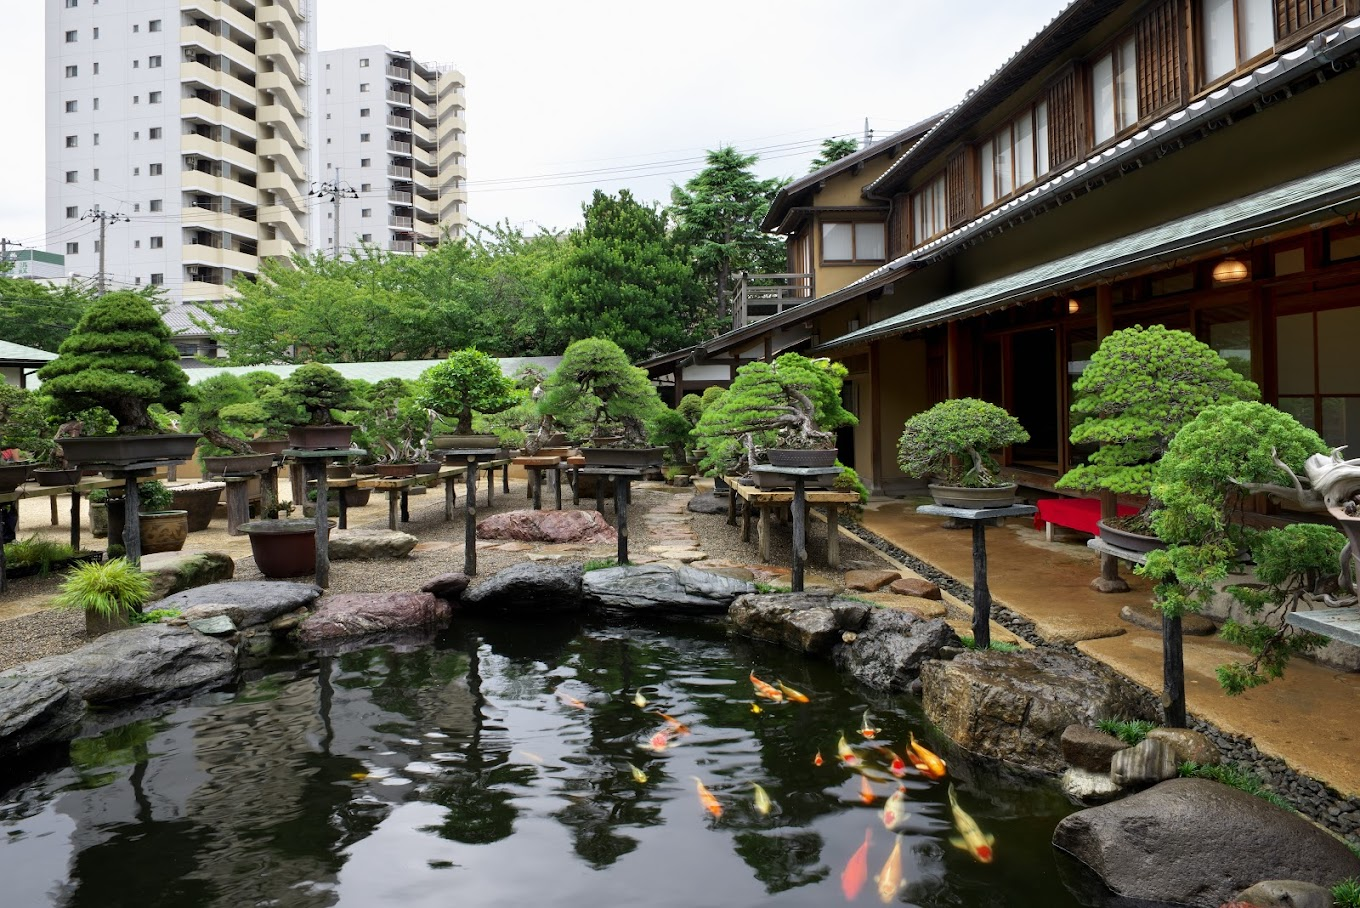
\includegraphics[width=1.0\columnwidth]{2025_11/res/opportunity_shunka-en_bonsai.jpg},\centerline{\emph{Shunka-en Bonsai Museum main garden.}}]
\end{window}

\closearticle
\columnbreak